\section{Electrical and Wiring}

	\begin{figure}[h]
		\centering
		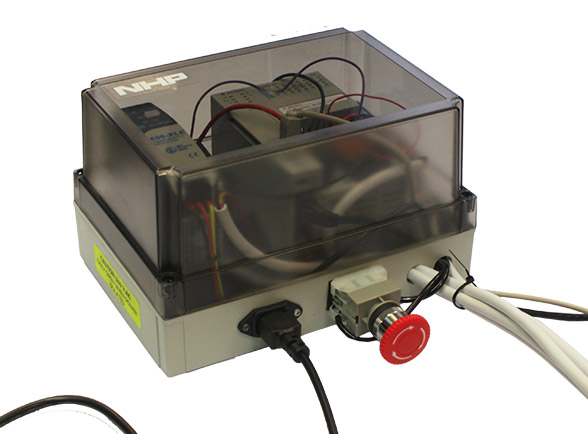
\includegraphics[width=0.5\textwidth]{figures/cncMachine/control.jpg}
		\caption{DoodleBot Control Enclosure}
		\label{fig:control}
	\end{figure}
	
	The wiring diagram in Figure ~\ref{fig:WiringDiagram} shows electrical layout of the system. The DoodleBot has two major groups of components - the electronics and control components sit in the DoodleBot Control Enclosure (Figure ~\ref{fig:control}) and the electromechanical components are mounted to the DoodleBot CNC Frame (Figure ~\ref{fig:implementation-mechanical}).

	
\begin{landscape}
		\vspace*{\fill}
		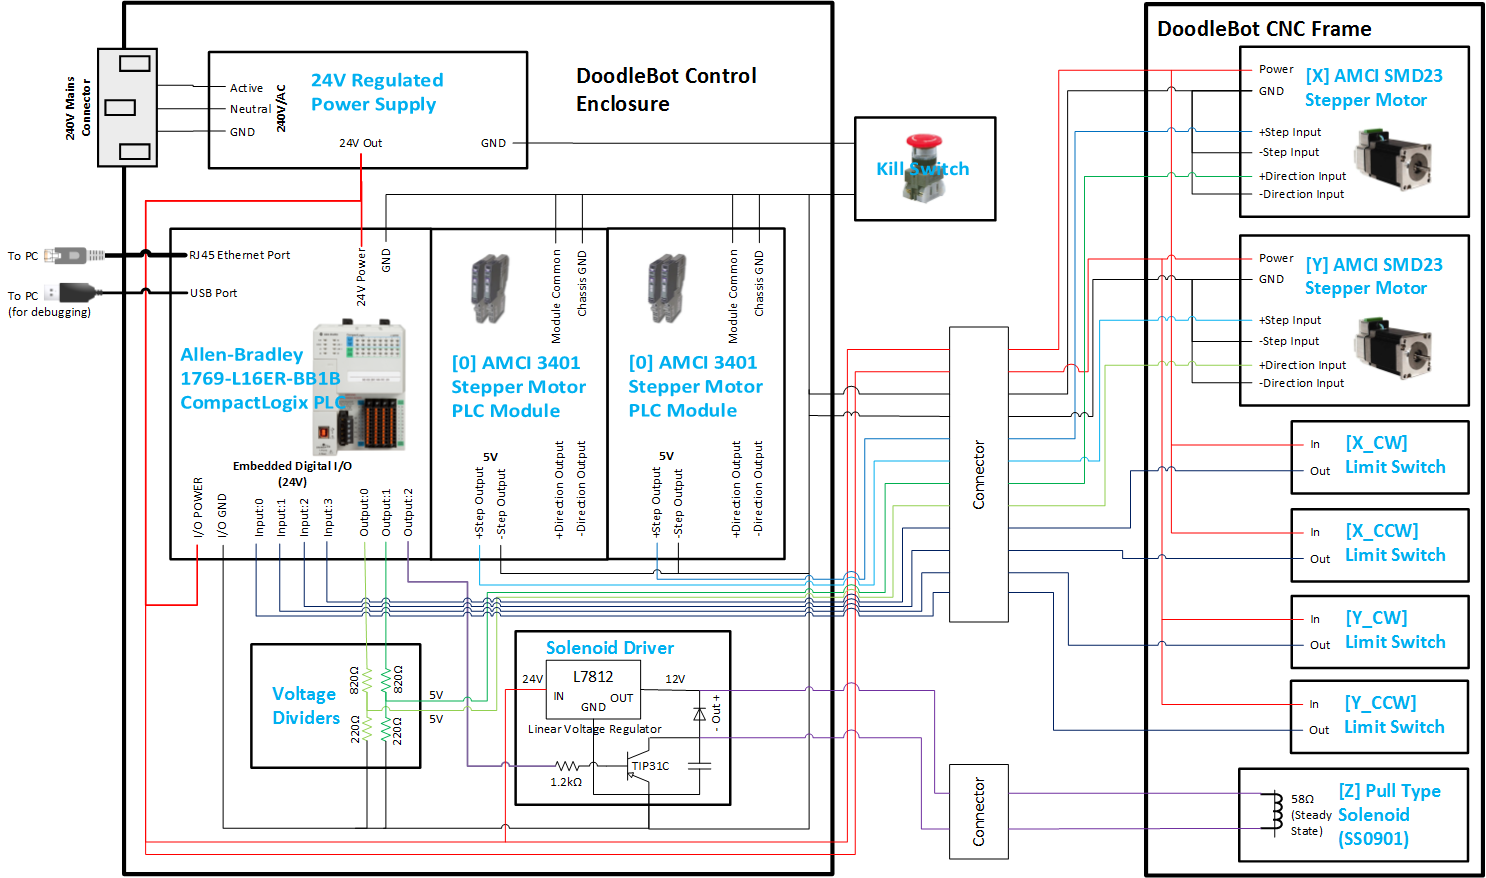
\includegraphics[width=\hsize]{figures/cncMachine/wiring}
		\captionof{figure}{Wiring Diagram}
		\label{fig:WiringDiagram}
		\vspace*{\fill}
\end{landscape}


	\subsection{Connectors and Loom}
	
	The DoodleBot team constructed a 14-wire loom to transmit power and signals between the Control Enclosure and the CNC Frame. Figure ~\ref{fig:loom} shows the plastic connector pin outs and Table ~\ref{table:loom} lists the details of each wire/pin in the loom.
		\begin{figure}[h]
			\centering
			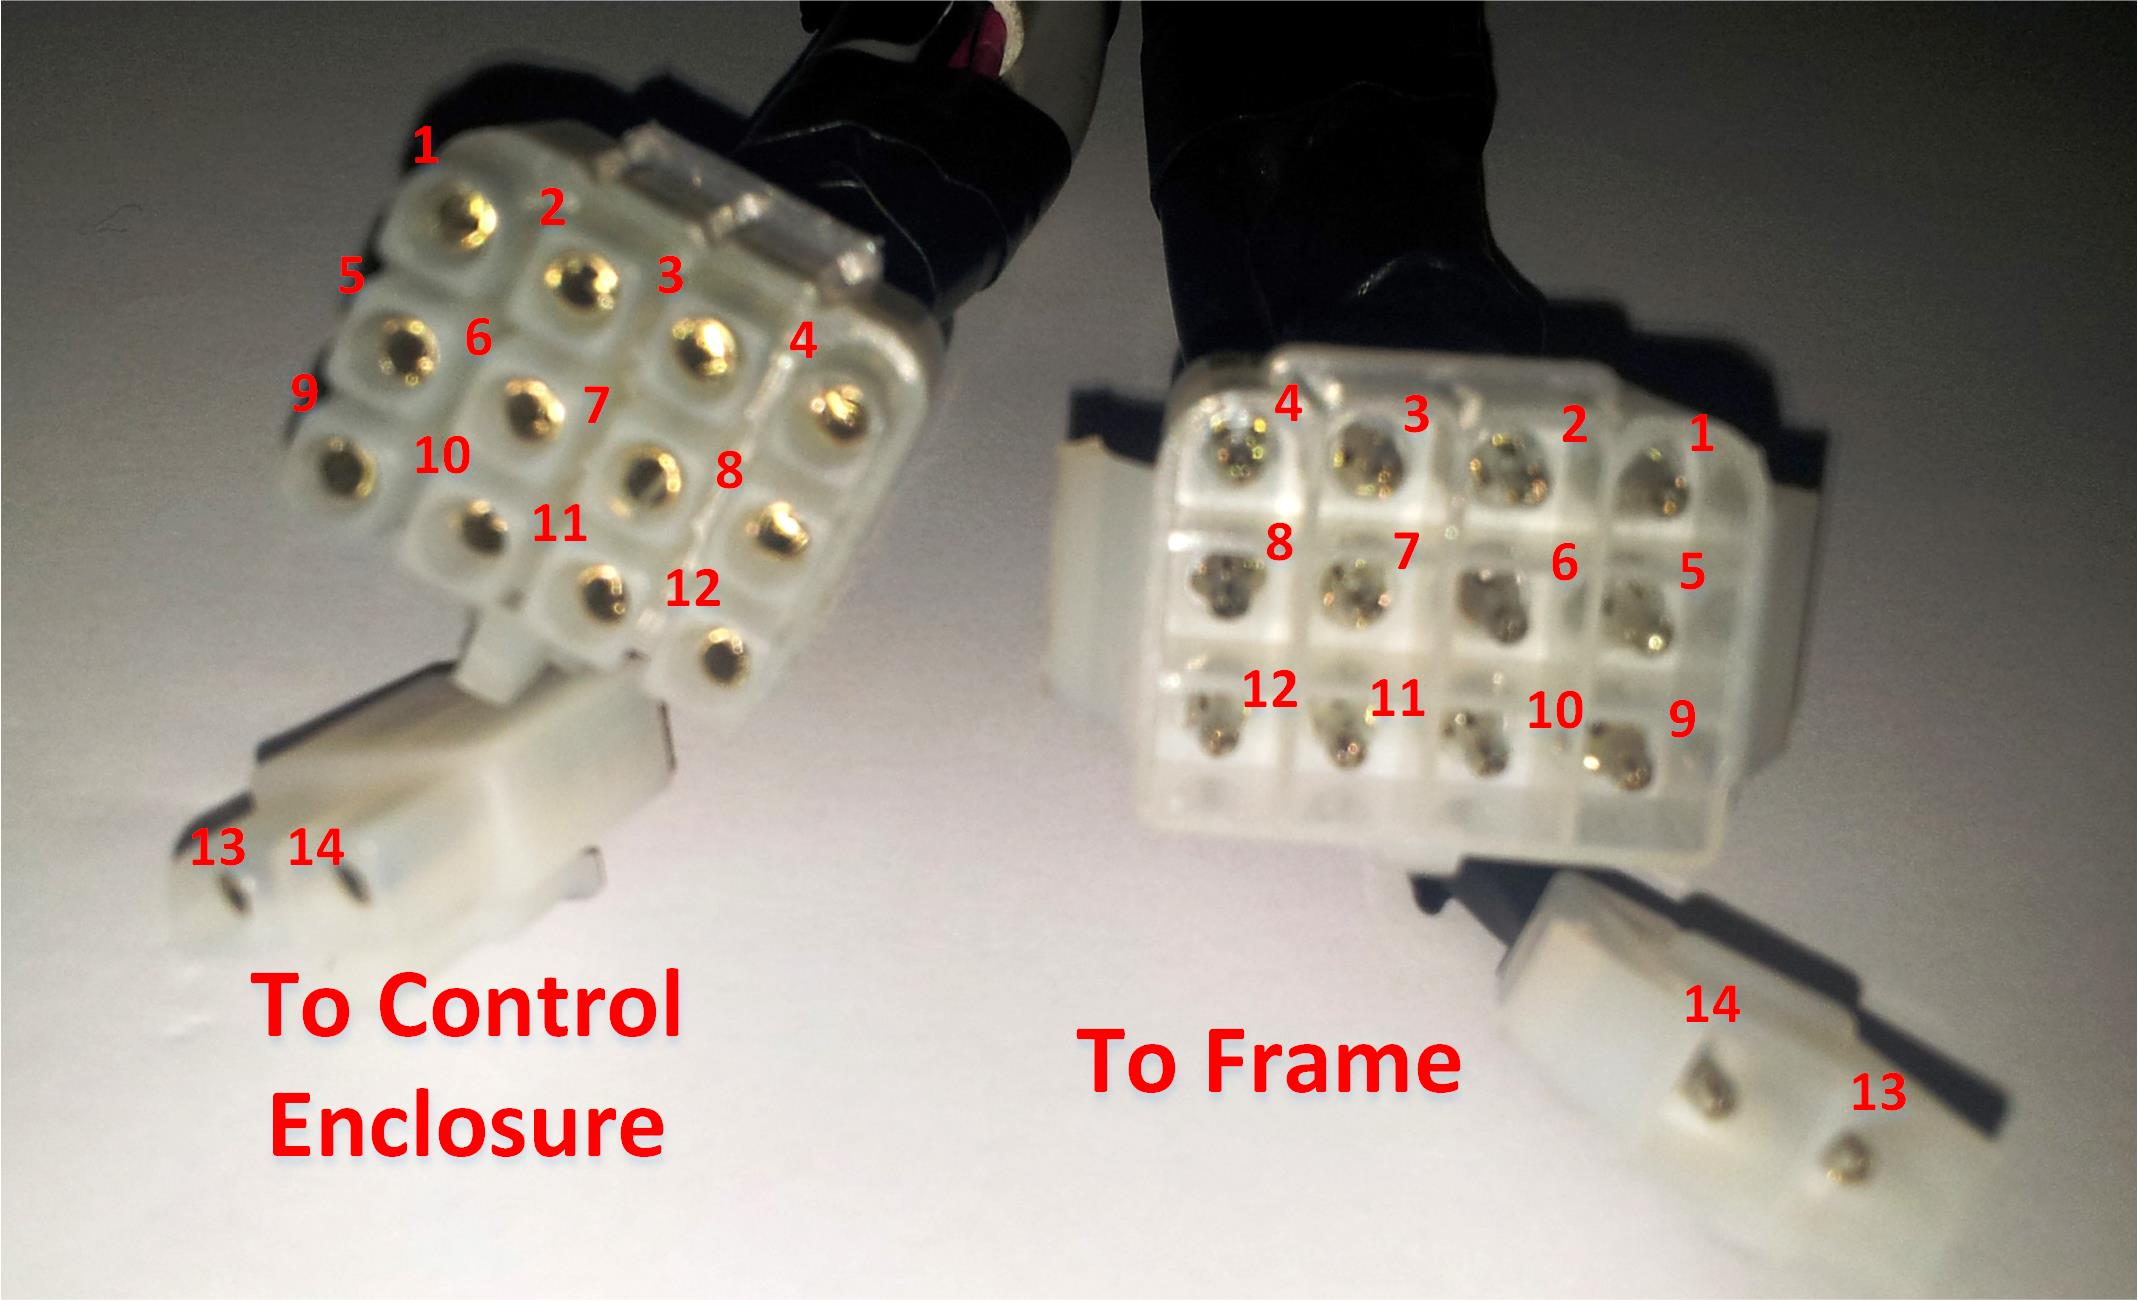
\includegraphics[width=0.5\textwidth]{figures/cncMachine/loom.jpg}
			\caption{Wiring Loom Connector Pin out}
			\label{fig:loom}
		\end{figure}
		
		\begin{table}[h]
			\centering
			\begin{tabular}{|c|c|c|l|l|}
				\hline
				\emph{Pin} & \emph{Wire Colour} & Voltage & \emph{Control Enclosure Side} & \emph{CNC Frame Side} \\ \hline
				1 & Red & 24V & Power & \parbox[t]{6cm}{SMD23 +PWR [X] \\ Limit Switch [X\_CW],[X\_CCW]} \\ \hline
				2 & Red/Yellow & 5.1V & PLC DC Output 0 & SMD23 +Direction [X]\\ \hline
				3 & Red & 5V &  3401 Step Output [0] & SMD23 +Step [X]\\ \hline
				4 & Black & 0V & GND & SMD23 -PWR, -Direction, -Step [X] \\ \hline
				5 & Red/Yellow & 24V & Power & \parbox[t]{6cm}{SMD23 +PWR [Y]\\ Limit Switch [Y\_CW],[Y\_CCW]}\\ \hline
				6 & Black/Yellow & 5.1V & PLC DC Output 1 & Stepper Motor Direction [Y]\\ \hline
				7 & Black & 5V &  3401 Step Output [1] & SMD23 +Step [Y]\\ \hline
				8 & Black/Yellow & 0V & GND & SMD23 -PWR, -Direction, -Step [Y] \\ \hline
				9 & Black & 24V & PLC DC Input 0 & Limit Switch [X\_CW]\\ \hline
				10 & Black/Yellow & 24V & PLC DC Input 1 & Limit Switch [X\_CCW]\\ \hline
				11 & Red & 24V & PLC DC Input 2 & Limit Switch [Y\_CW]\\ \hline
				12 & Red/Yellow & 24V & PLC DC Input 3 & Limit Switch [Y\_CCW]\\ \hline
				13 & Red/Yellow & 12V & +Solenoid Driver Output & +Solenoid [Z]\\ \hline
				14 & Black & 0V & -Solenoid Driver Output & -Solenoid[Z]\\ \hline
			\end{tabular}
			\caption{Wiring loom and connector specifications}
			\label{table:loom}
		\end{table}
	\subsection{Voltage Dividers}
		The direction signals for the stepper motors are produced from the PLC on pins $embedded.DCout.0$ and $embedded.DCout.1$ at $24V$. The AMCI SMD23 only accepts a differential input of $5V$.
		
		Since the AMCI SMD23 direction input is a digital signal (ie, high impedance input), we can use a simple voltage divider circuit to produce the correct voltage. 
		
		The PLC embedded output can produce a maximum of $500mA$ per pin. One important thing to consider however, is it requires a \emph{minimum} of $1mA$ from each pin while in the on-state to operate properly. 
		
		Choosing resistors of $820\Omega$ and $220\Omega$ in the voltage dividers give a $5.08V$ output and draw $2.3mA$, satisfying the minimum current condition. 
	\subsection{Solenoid Driver}
		A Jaycar SS0901 pull-type solenoid is used to control the drawing head operation.
		
		The solenoid is designed to operate at $12V$, has a resistance of $58\Omega$ and an unknown inductance. In steady state operation it draws $207mA$ and consumes $6W$. The solenoid can be modelled as an R-L circuit: an off-on transition will begin with current draw of $0mA$ and transiently approach $207mA$. In an on-off transition, there will be a large spike of negative current which gradually reduces to zero as the inductor component discharges.
		
		The PLC embedded output can produce a maximum of $500mA$ per pin. One important thing to consider however, is it requires a \emph{minimum} of $1mA$ from each pin while in the on-state to operate properly. 
		
		Due to the transient behaviour of the solenoid, a simple voltage divider cannot be used. Instead an STMicroelectronics L7812 Linear Voltage Regulator in TO220 packaging is used to perform the $24V-12V$ DC-DC conversion. $6W$ of power is lost as heat in the L7812 during the on-state and so a heatsink is used and the housing for the circuit is vented.
		
		Due to the minimum current requirement of the PLC output, a TIP31C bipolar junction transistor (BJT) is used as the solenoid switch. A field effect transistor (FET) would not work since it would not draw enough current to allow the PLC output to operate properly.
		
		To meet the $207mA$ required by the solenoid, there is a minimum current requirement through the base of the BJT. The TIP31C datasheet shows that tested with a collector-emitter current of 1A, the minimum DC current gain is 25. So at least $8.28mA$ is required through the base. A more conservative value of $20mA$ is chosen by placing a $1.2k\Omega$ resistor in between the PLC output and BJT base.
		
		To allow the inductor to discharge quickly (and without damaging other components), a flyback switching power diode is put across the Solenoid Driver Output in reverse orientation. In the on-off transition, the inductor discharge current (flowing in the reverse direction of normal current flow) will have an alternate path to follow and energy will dissipate as heat in the solenoid and diode. This protects other electronic components as well allowing the solenoid to be more responsive in dropping its load.
		
	\subsection{Kill Switch}
		The DoodleBot features a kill switch (emergency stop switch) mounted to Control Enclosure that disconnects the power supply's GND output from all the powered components. 
		
		It should be noted that the power supply itself continues to operate and energy storage components in the rest of the circuit (eg, inductors and capacitors) will retain their charge.


